%%%%% Kompendium -- Wellen und Optik %%%%%
%% Schwingungen %%


%Some sample text to be displayed above the first subsection

%\subsection{Prinzip}

%Ein Zyklotron besteht aus Zwei hohlen, halbzylindrischen und Duanden an denen eine Spannung mit unterschiedlichem Vorzeichen anliegt, und darüber bzw. darunter liegende Magneten, die ein homogenes Magnetfeld erzeugen. Zudem gibt es einen Einlass und einen Auslass für Teilchen.

%\begin{wrapfigure}{r}{0.4\textwidth} \label{Zyklo}
%
%	\vspace{-10pt}
%	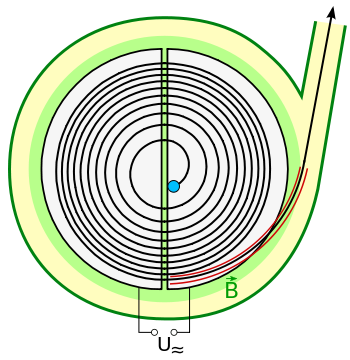
\includegraphics[width=0.35\textwidth]{Zyklotron_Prinzipskizze02.png}
%	\vspace{-13pt}
%	\caption{Prinzipskizze eines Zyklotrons}
%	\vspace{-5pt}	
%	
%\end{wrapfigure}

%\subsubsection{Anwendung}

% Some Formula:

%\begin{equation}
%	x= \frac{y \cdot 13 \pi z}
%			{\cos \alpha}
%\end{equation}

%%%%%%%%%%%%%%%%%%%%%%%
% Eigentlicher Beginn %
%%%%%%%%%%%%%%%%%%%%%%%


\subsection{Diagramm einer Schwingung} \label{subsec:diagramm_schwingung}

\begin{figure}[h!]


	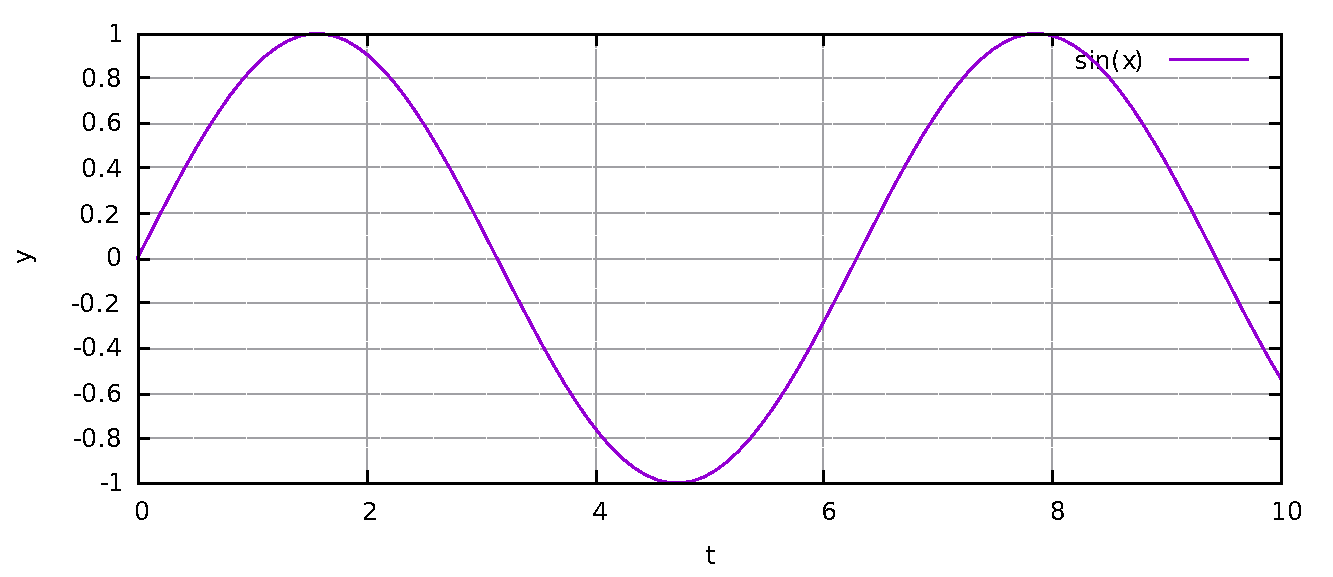
\includegraphics[width=0.9\textwidth]{Pictures/schwingung}

	\caption{Diagramm einer Schwingung: Elongation über der Zeit}

	
\end{figure}

\subsection{Kenngrößen von Schwingungen} \label{subsec:kenngroessen_schwingungen}


\subsubsection[Amplitude]{Amplitude: $y_{max}$ o. $s_{max}$ o. $\hat{y}$ o. $\hat{s}$ (Basiseinheit: $m$)}

Die maximale Elongation (=\glqq Auslenkung\grqq) der Schwingung.


\subsubsection[Periodendauer]{Periodendauer: $T$ (Basiseinheit: $s$)}
	
Die Zeit, die es dauert bis der schwindende Körper an der selben Stelle von der selben Richtung aus angelangt ist. Beispielsweise vom positiven Schwingungsmaximum (\glqq Berg\grqq) zum nächsten oder von der Nullstelle (\glqq Ruhelage\grqq) zur 2. darauffolgenden Nullstelle.

Davon abgeleitet:
\begin{itemize}
	\item Frequenz: $f=\frac{1}{T}$ (Basiseinheit: $Hz=\frac{1}{s}$)
	
	Anzahl der Perioden pro Sekunde.
	\item Winkelgeschwindigkeit: $\omega=2 \pi f=\frac{2 \pi}{T}$ (Basiseinheit: $\frac{rad}{s}$)
		
	Änderung des Winkels über der Zeit, wobei eine ganze Periode mit $360 \degree$ im Grad oder, im Physikunterricht verwendet, mit $2 \pi$ im Bogenmaß (eng: \glqq Radian\grqq) bezeichnet wird.\footnote{Umrechnung des Winkels $\alpha$ von Grad nach Bogenmaß: $\alpha_{rad} = \alpha_{deg} \cdot \frac{2\pi}{360 \degree} = \alpha_{deg} \cdot \frac{\pi}{180 \degree} $}
\end{itemize}


\subsubsection[Phasenverschiebung]{Phasenverschiebung: $\phi$ (Basiseinheit: $rad$)}
	
Wenn sich der Schwingungskörper zum Startzeitpunkt $t=0$ nicht in der Ruhelage $y=0$ befindet muss die Phasenverschiebung, z.B. zur Aufstellung der Schwingungsgleichung (\referenz{subsec:schwingungsgleichungen}), berücksichtigt werden. Die Phasenverschiebung gibt den Abstand von der y-Achse zum nächsten Durchlauf der Ruhelage von der negativen Seite.

	\begin{wrapfigure}{r}{0.5\textwidth} \label{phasenverschiebung}
	
		\vspace{-10pt}
		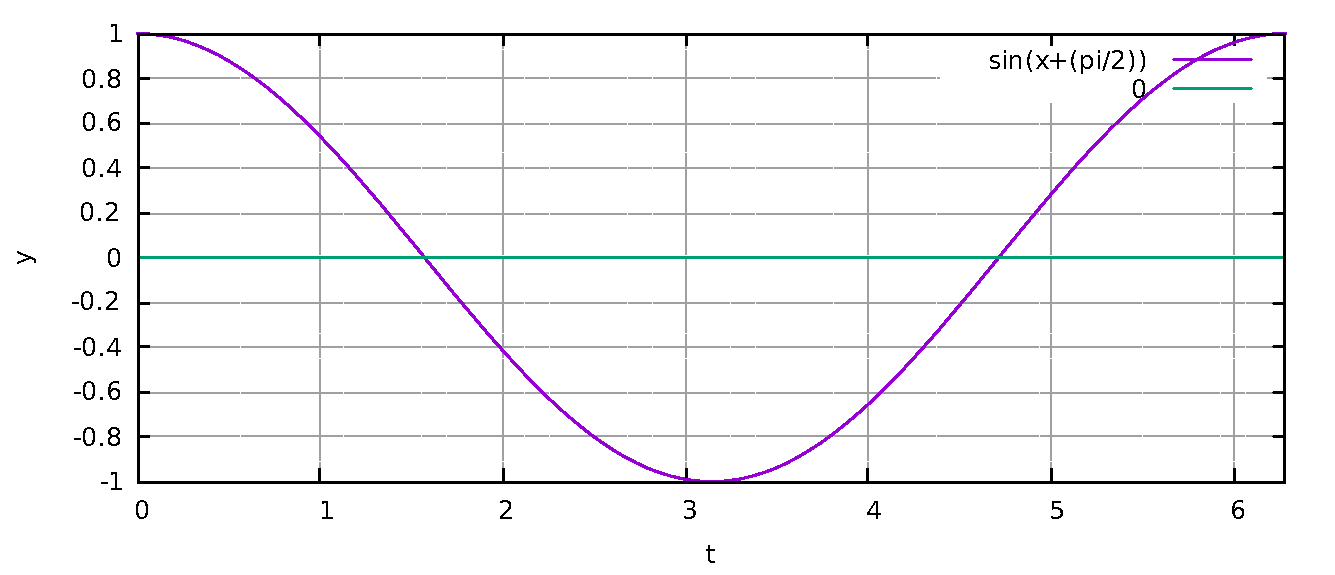
\includegraphics[width=0.48\textwidth]{Pictures/phasenverschiebung}
		\vspace{-13pt}
		\caption{Phasenverschiebung um $+\frac{3\pi}{2}$}
		\vspace{-5pt}
	
	\end{wrapfigure}

Im nebenstehenden Diagramm beträgt die Phasenverschiebung $\phi = +\frac{3\pi}{2}$, also ein Drei-Viertel der Periode. Man könnte ebenfalls sagen, die Phasenverschiebung beträgt $\phi = -\frac{\pi}{2}$, also minus Ein-Viertel der Periode. Beides ist äquivalent, jedoch ist es leichter mit einer positiven Phasenverschiebung zu rechnen.
	
	


\subsection{Schwingungsgleichungen} \label{subsec:schwingungsgleichungen}

Daraus ergibt sich folgende Schwingungsgleichung, bzw. Schwingungsfunktion, für eine harmonische Schwingung (\referenz{sec:definitionen}), die die Elongation in Abhängigkeit der Zeit angibt:

\begin{equation} \label{eq:schwingungsgleichung_y}
	y(t)=y_{max} \cdot \sin{(\omega t + \phi)}
\end{equation}

Die erste Ableitung dieser Gleichung nach $t$ gibt die Geschwindigkeit des Schwing-körpers zur Zeit $t$ an:

\begin{equation} \label{eq:schwingungsgleichung_v}
	y'(t)=v(t)=y_{max} \cdot \omega \cdot \cos{(\omega t + \phi)}
\end{equation}

Die zweite Ableitung gibt die Beschleunigung des Schwingkörpers zur Zeit $t$ an:

\begin{equation} \label{eq:schwingungsgleichung_a}
	y''(t)=v'(t)=a(t)=y_{max} \cdot \omega^{2} \cdot -\sin{(\omega t + \phi)}
\end{equation}


\subsection{Weitere Gleichungen und Gesetze}

\subsubsection{Gesetze im Kreis}

\paragraph{Bahngeschwindigkeit im Kreis}

Die Bahngeschwindigkeit gibt in absoluten Einheiten ($\frac{m}{s}$) an, wie schnell sich das Objekt auf der Bahn fortbewegt. Zusätzlich zur Winkelgeschwindigkeit (\referenz{subsec:kenngroessen_schwingungen}) muss bei der Kreisbahn daher noch der Radius bekannt sein:

\begin{equation*} \label{eq:bahngeschwindigkeit}
	v=\frac{2r\pi}{T}=\omega r
\end{equation*}

Eine andere Herleitung aus dem Kreisumfang $U=2r\pi$, der Periodendauer $T$ und der generellen Formel für Bahngeschwindigkeit $v=\frac{s(t)}{t}$ könnte wie folgt Aussehen:

\begin{align*}
	v&=\frac{s(t)}{t} \\
	v&=\frac{2r\pi}{T}
\end{align*}


\paragraph{Zentripetalbeschleunigung}

Um auf einer Kreisbahn zu bleiben, muss eine Zentripedalbeschleunigung auf einen Körper wirken, die zum Kreiszentrum hin zeigt. Die Formel lautet:

\begin{equation*}
	a_z=\frac{v^2}{r}=\omega^2 r
\end{equation*}


\paragraph{Zentripetalkraft}

Dies ist die Kraft, die auf einen Körper ausgewirkt werden muss, damit er auf einer Kreisbahn bleibt. Zusätzlich zur Zentripetalbeschleunigung muss nun also noch gemäß Newtons zweiten Axiom $F=a \cdot m$ die Masse als Faktor in die Gleichung aufgenommen werden:

\begin{align*}
	F_z &= a_z \cdot m \\
	F_z &= \frac{v^{2}m}{r}
\end{align*}


\subsubsection{Gesetze bei Geschwindigkeiten}

Aus der maximalen Geschwindigkeit und der Frequenz, Periodendauer oder Winkelgeschwindigkeit lässt sich sofort auf die Amplitude schließen, da in der Funktion für die Geschwindigkeit bei einer Schwingung (\referenz{subsec:schwingungsgleichungen}) $v(t)=\omega \cdot y_{max} \cdot \cos{(\omega t)}$ das Maxima dann erreicht ist, wenn der Cosinus seinen Maximalwert $1$ annimmt. Dann gilt folgendes:

\begin{align*} \label{eq:geschwindigkeit_amplitude}
	v_{max} &= \omega \cdot y_{max} \\
	v_{max} &= 2\pi f \cdot y_{max} \\
	y_{max} &= \frac{v_{max}}{2\pi f}
\end{align*}


\subsubsection{Gesetze am Federpendel}

\paragraph{Hooke'sches Gesetz}

Das Hooke'sche Gesetz gibt die Federhärte einer Feder, also dessen Kenngröße, an. Die Einheit $\frac{N}{m}$ erklärt selbst die Formel:

\begin{equation*}
	D=\frac{F}{l}
\end{equation*}

Mit dem Gesetz ist gezeigt, dass an einem Federpendel die Rückstellkraft $F$ proportional zur Auslenkung $l$ ist. Damit ist es eine harmonische Schwingung. (\referenz{subsec:definitionenzuschwingungen})

\paragraph{Periodendauer beim Federpendel}

Die Periodendauer beim Federpendel ist abhängig von der Masse $m$ und der Federkonstante $D$:

\begin{equation*}
	T_{Feder}=2\pi \cdot \frac{m}{D}
\end{equation*}

Die Herleitung gestaltet sich folgendermaßen: Die zur Auslenkung $y$ proportionale Kraft $F$ ist die Rückstellende Kraft; beschrieben durch eine Umformung des Hooke'schen Gesetzes: $F_{r}=D \cdot y$. 
%Der Vektor dieser Rückstellende Kraft zeigt dem der Auslenkenden Kraft genau entgegen, daher muss der Term in diesem Fall negiert werden: $F_{r}=-D \cdot y$.

In einem geschlossenen System ist die Summe aller Kräfte $0$. Es ergibt sich Folgendes:

\begin{align*}
	F_a + F_r &= 0 \\
	F_a &= -F_r \\
\end{align*}

Die Kraft $F_a$ kann wie jede Kraft mit Newtons zweitem Gesetz als $F_a=m \cdot a$ beschrieben werden. Die Beschleunigung in $a$ kann dann als zweite Ableitung der Auslenkung $y$ nach der Zeit beschrieben werden. Aus den Schwingungsgleichungen (\referenz{subsec:schwingungsgleichungen}) geht hervor, dass $y''=-\omega^{2} \cdot y$ ist. Daher kann man wie folgt einsetzen:

\begin{align*}
	m \cdot a &= -D \cdot y \\
	m \cdot y'' &= -D \cdot y \\
	m \cdot -\omega^{2} \cdot y &= -D \cdot y \\
	- m \cdot \omega^{2} &= -D \\
	\omega &= \sqrt{\frac{D}{m}}
\end{align*}

Für aus $\omega=\frac{2\pi}{T}$ folgt für $T$:

\begin{equation*}
	T = 2\pi \cdot \sqrt{\frac{m}{D}}
\end{equation*}











